\documentclass{article}
\usepackage{tikz}
\usepackage{tikz-feynman}
\usepackage[utf8]{inputenc}

\begin{document}

The $W$ boson is not only an important force carrier, it is also the mediator between subatomic decays. For example, you'll see that the $W$ boson has a role to play in muon decay or in the flavor change of quarks. Why is flavor change important? Well, it happens very often in neutron decay or proton-electron collisions as you'll see below!


Below, we'll look at a muon decaying into a muon neutrino and an electron. We'll also look at cases where a proton will decay into a neutron (via positron emission) or the case where a neutron may become a proton and an electron (via beta emission).

The figure below shows a muon decaying via a $W^-$ boson into a muon neutrino. Notice that the $W^-$ boson will then decay into an electron and electron neutrino.

Recall for a moment that the mass of a muon is 105.66 MeV and an electron's mass is 0.511 MeV. You might see then that it is completely possible for a muon at rest to decay into an electron.

Rememver that by the conservation of momentum, the momentum of $e^{-}$ and $\overline{\nu}_{e}$ will be equal and opposite. We might surmise that the neutrino will be going much faster than the electron in this case. Let's delve a little deeper using Einstein's Energy-Momentum relation.
% Muon decay diagram
\begin{figure}[h]
    \centering
    \resizebox{20em}{!}{
        \begin{tikzpicture}
            \begin{feynman}
                \vertex (a) {\(\mu^{-}\)};
                \vertex [right=of a] (b);
                \vertex [right=of b] (c) {\(\nu_\mu\)};
                \vertex [above right=of b] (d);
                \vertex [right=of d] (f) {\(\overline{\nu}_{e}\)};
                \vertex [above right=of d] (e) {\(e^{-}\)};
                \vertex [above=2.0em of b] (W);
                \vertex [right=-0.5em of W] (fW) {\(W^-\)};

                \diagram* {
                    (a) -- [fermion] (b) -- [fermion] (c),
                    (b) -- [boson] (d),
                    (d) -- [fermion] (f),
                    (d) -- [fermion] (e),
                };
            \end{feynman}
        \end{tikzpicture}
    }
    \caption{Muon decay via the $W^- boson$}\label{fig:C1-1}
\end{figure}

% Quark flavor change diagram
\begin{figure}[h]
    \centering
    \resizebox{20em}{!}{
        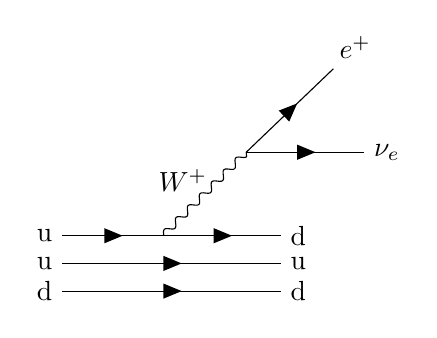
\begin{tikzpicture}
            \begin{feynman}
                \vertex (a) {u};
                \vertex [right= of a] (b);
                \vertex [right= of b] (c) {d};
                \vertex [below=1em of a] (qu1) {u};
                \vertex [below=1em of c] (qu2) {u};
                \vertex [below=1em of qu1] (qd1) {d};
                \vertex [below=1em of qu2] (qd2) {d};

                \vertex [above right= of b] (d);
                \vertex [right= of d] (f) {\(\nu_e\)};
                \vertex [above right= of d] (e) {\(e^+\)};

                \vertex [above=2.0em of b] (W);
                \vertex [right=-0.5em of W] (fW) {\(W^+\)};

                \diagram* {
                    (a) -- [fermion] (b) -- [fermion] (c),
                    (qu1) -- [fermion] (qu2),
                    (qd1) -- [fermion] (qd2),

                    (b) -- [boson] (d),
                    (d) -- [fermion] (f),
                    (d) -- [fermion] (e),
                };
            \end{feynman}
        \end{tikzpicture}
    }
    \caption{Proton becomes a neutron by emitting a positron.}\label{fig:C1-2}
\end{figure}

Bear in mind that there is a very similar process when the reverse happens (a neutron will decay into an electron and a proton).

\begin{figure}
    \centering
    \resizebox{20em}{!}{
        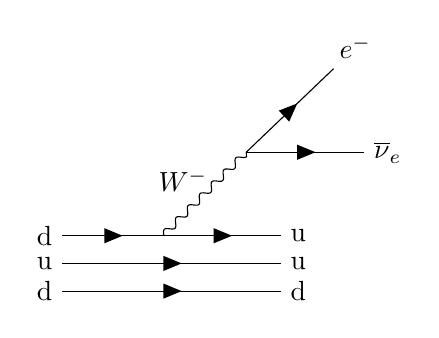
\begin{tikzpicture}
            \begin{feynman}
                \vertex (a) {d};
                \vertex [right= of a] (b);
                \vertex [right= of b] (c) {u};
                \vertex [below=1em of a] (qu1) {u};
                \vertex [below=1em of c] (qu2) {u};
                \vertex [below=1em of qu1] (qd1) {d};
                \vertex [below=1em of qu2] (qd2) {d};

                \vertex [above right= of b] (d);
                \vertex [right= of d] (f) {\(\overline{\nu}_e\)};
                \vertex [above right= of d] (e) {\(e^-\)};

                \vertex [above=2.0em of b] (W);
                \vertex [right=-0.5em of W] (fW) {\(W^-\)};

                \diagram* {
                    (a) -- [fermion] (b) -- [fermion] (c),
                    (qu1) -- [fermion] (qu2),
                    (qd1) -- [fermion] (qd2),

                    (b) -- [boson] (d),
                    (d) -- [fermion] (f),
                    (d) -- [fermion] (e),
                };
            \end{feynman}
        \end{tikzpicture}
    }
    \caption{Neutron becomes a proton through emitting an electron}\label{fig:C1-3}
\end{figure}

\begin{equation}
    (i\gamma^{\mu} \partial_{\mu} - m)\psi = 0.
\end{equation}  

\end{document}

